% ------------------------------------------------------------------
%   The basic memos for the standard model of particle physics
%   and SU(5) Grand Unified Theory 
%
%   Last Modified: Feb 29 2025
%   Author: Yasutoki Takamura
%   Kanazawa University / Institute of theoretical particle physics
% ------------------------------------------------------------------
\RequirePackage{plautopatch}
\documentclass[uplatex,dvipdfmx,a4paper,titlepage,10pt]{jsreport}


% ----- preambles ------------------
\usepackage{geometry}
\usepackage{bm}
\usepackage{here}
\usepackage{amsmath,amsthm,amssymb}
\usepackage{ascmac}
\usepackage{cite}
\usepackage{color}
\usepackage{comment}
%\usepackage{multibib}
\usepackage[dvipdfmx]{graphicx}
%\usepackage{etoolbox}
%\apptocmd{\sloppy}{\hbadness 10000\relax}{}{}
\usepackage{tikz}
\usetikzlibrary{tikzmark}
\usepackage[compat=1.1.0]{tikz-feynhand}
\usepackage[dvipdfmx]{hyperref}
\usepackage{pxjahyper} % (u)pLaTeXのときのみかく
\hypersetup{%
 setpagesize=false,%
 bookmarksnumbered=true,%
 colorlinks=true,%
 pdftitle={},%
 pdfsubject={},%
 pdfauthor={},%
 pdfkeywords={},%
 hidelinks,%
 citecolor=blue,%
 filecolor=blue,%
 urlcolor=blue,%
 linkcolor=blue,
 }
% ----------------------------------


% ----- Settings for amsthm -----
\theoremstyle{plain}
\newtheorem{thm}{Theorem}
\newtheorem*{thm*}{Theorem}

\theoremstyle{definition}
\newtheorem{dfn}{Definition}
% -------------------------------


% ----- Geometry setting ---------------------------
\geometry{left=25mm,right=25mm,top=25mm,bottom=30mm}
\begin{document}


% ----- Title Page -------------
\title{SU(5)大統一理論における15表現ヒッグスを用いた模型の拡張}
\author{金沢大学大学院\,\,自然科学研究科数物科学専攻\,(物理学コース)修士課程2年\\学籍番号\,2315011026$\quad$名列番号216\\高村 泰時} 
\date{\today}
\maketitle

% ----- Contents page -------------------------------
\tableofcontents
\clearpage

% ----- Abstract ------------------------------------
\begin{abstract}
素粒子標準模型とは, $SU(3)_c\times SU(2)_L\times U(1)_Y $ ゲージ群によって素粒子の相互作用を記述する理論であり, 素粒子がもたらす実験や観測を非常によく説明する.
ところが標準模型では説明できない現象も数多く存在する.
例えば, 標準模型ではニュートリノには質量が存在しないが, カミオカンデでニュートリノ振動が観測され, ニュートリノに質量が存在することが明らかにされた.
他にも様々な側面から標準模型を超えた理論への拡張が迫られており, 大統一理論はその候補の一つとして挙げられる.

大統一理論とは, 標準模型のゲージ軍を部分群として含む単純群によって構成され, 物質粒子やゲージ粒子を統一的に記述する.
標準模型では陽子と電子の電荷が量子化されていないことを理論的に説明することができないが, 大統一理論によって理論的な説明がなされるため, 大統一理論を研究する大きな動機となる.
相互作用が統一的に記述されるため, 高いエネルギースケールでは相互作用の大きさも統一されるべきと考えるが, H.GeorgiとS.L.Glashowによって初めて考案された$SU(5)$大統一模型はゲージ結合定数の統一は叶わず, また標準模型でも課題であったニュートリノ質量を説明することはできなかった.
そのため, $SU(5)$大統一理論を実現するためには$SU(5)$ゲージ群の枠組みの中で理論を拡張することで, 標準模型の課題を解決できる整合性の取れた理論にする必要がある.
本論文では初めに標準模型のレビューを行い, 実験的にどのような課題が存在するのかをまとめた.
また, 標準模型を大統一理論へ拡張するために$SU(5)$大統一理論の一般的な構築を行った.
最後に, 最小$SU(5)$模型ではゲージ結合定数の大きさが統一することができないことを受け, I.Dorsnerらが行った最小$SU(5)$大統一理論に対して$\bm{15}$表現ヒッグスを拡張する模型を再現した.
これによりゲージ結合定数の大きさが大統一スケールで近づくことを確認した.
\end{abstract}

% =========================
% ----- Main Contents -----
% =========================
% ----- 1st part -----
%\part{教科書の部分}

\chapter{記法}
$B$3$NK\$GMQ$$$k5-K!$K$D$$$F$O<!$N$b$N$K$7$?$,$&(B.
$B?o;~99?7$9$k$3$H(B.


\chapter{素粒子標準模型}
% ---------------------------------------
%
%  Standard model
%  Standard_Model.tex
%  Program modified by Yasutoki Takamura
%  Last Modified Nov 29 2024
%
% ---------------------------------------
この章では素粒子物理学における標準模型についてまとめた.
素粒子標準模型は現在の高エネルギー実験をほぼ説明することができるものであるが, 標準模型だけでは説明できない事実が存在する.
大統一理論はそれらを解決するための理論の一つであるが, そもそも標準模型がどのような理論であるのかをここで振り返る.
\subsection{概観}
素粒子標準模型は量子場の理論により記述される.
素粒子の相互作用はYang-Millsによる理論によって, 数学的にリー群に属する局所非可換ゲージ変換のもとで不変になるようにラグランジアン密度を記述することができる.
具体的には, 次のようなゲージ対称性を持つ理論である.
\begin{align}
  \mathcal{G}_{\text{SM}}\mathrm{SU}_\mathrm{c}\times \mathrm{SU}_\mathrm{L}\times \mathrm{U}(1)_\mathrm{Y}\label{SM-Gauge}
\end{align}
それぞれゲージ群の添字は量子数に対応している.
"C"はカラー量子数, "L"は左巻きのカイラリティ, "Y"は超電荷である.
$\mathrm{SU}3_c$群は核子にはたらく強い相互作用を記述する群であり, 量子色力学(QCD)によって記述される.
一方で$\mathrm{SU}(2)_L\times \mathrm{U}(1)_Y$は弱い相互作用と電磁相互作用を統一的に記述する電弱理論を記述する群である.

ゲージ対称性の他に, 理論に現れる粒子がどのようなものであるのか, 標準模型のゲージ対称性の中でどのような対称性を持つ粒子であるのかを決めることにより, 理論を具体的に決定することができる.
他にも, ラグランジアン密度に含める項は, 繰り込み可能であり, ローレンツ対称性を満足するものを決めることで全て書き下すことができる.
以下では, 標準模型に現れる粒子について具体的に記述をする.
\subsection{ゲージ粒子}
\subsection{フェルミオン}
\subsection{ゲージ理論}
\subsection{ヒッグス機構}


%EOF

% ---------------------------------------
%
%  Some difficulties of Standard Model
%  SM_problems.tex
%  Program modified by Yasutoki Takamura
%  Last Modified Jul 18 2024
%
% ---------------------------------------
\section{標準模型の抱える問題}
素粒子標準模型は高エネルギー物理学の実験をほぼ正確に予言することができるため, 大きな成功を収めた.
特に2011年にCERNにある大型ハドロン衝突型加速器(Large Hadron Corrider; LHC)が標準模型に現れるHiggs粒子を発見したことにより, 標準模型は揺るぎないものとなった.
しかし, 次のような課題があり, 理論の拡張が迫られている.
\begin{itemize}
        \item ニュートリノ質量, およびニュートリノ振動\\
              標準模型ではニュートリノは質量を持たない粒子として存在する.
              しかし1998年にニュートリノ振動がスーパーカミオカンデで観測されたことにより, ニュートリノは質量を持つことが示唆されたため, 標準模型を何かしら拡張する必要があると考えられている.
      \item 重力相互作用
      \item 真の統一理論
      \item 電荷の量子化
      \item 階層性問題
      \item 予言できないパラメーターの数
      \item 暗黒物質
      \item 暗黒エネルギー
\end{itemize}
%EOF



\section{ニュートリノ質量}
%% ---------------------------------------
%
%  Neutrino Mass
%  neutrino.tex
%  Program modified by Yasutoki Takamura
%  Last Modified Dec 12 2024
%
% ---------------------------------------
$BAGN3;RI8=`LO7?$G$O(B, $B%K%e!<%H%j%N$K$O<ANL$,$J$$(B.
$B$3$l$O(B, $B%l%W%H%s%;%/%?!<$G$O%K%e!<%H%j%N$O(B$SU(2)_L$$BFs=E9`$K$N$_B8:_$7(B, $B%+%$%i%k%Q!<%H%J!<$G$"$k1&4,$-%K%e!<%H%j%N$,B8:_$;$:(B, $BB>$NN3;R$N$h$&$K%R%C%0%95!9=$r9M$($k$3$H$,$G$-$J$$$?$a$G$"$k(B.
$B$H$3$m$,(B, $B$9$G$K%+%_%*%+%s%G$K$h$k4QB,$K$h$j(B, $B%K%e!<%H%j%N?6F0$H8F$P$l$k%K%e!<%H%j%N$N%U%l!<%P!<$,JQ2=$9$k8=>]$,H/8+$5$l$?$3$H$+$i%K%e!<%H%j%N$K$b<ANL$,$"$k$H9M$($J$1$l$P$J$i$J$$(B.
\subsection{$B%^%h%J%i<ANL9`(B}
$B$3$3$G$O(B, $B%K%e!<%H%j%N$N<ANL9`$rF3F~$9$k$?$a$K%^%h%i%J>l$rF3F~$9$k(B.
$BNL;R>l$NM}O@$G$O(B, $B<ANL$r;}$C$?N3;R$O(B4$B@.J,$N%G%#%i%C%/%9%T%N!<%k>l$rMQ$$$F5-=R$5$l$F$$$?(B.
$B$3$N%G%#%i%C%/%9%T%N!<%k>l$r(B$\psi_D$$B$H$9$k(B.
$B%G%#%i%C%/%9%T%N!<%k$H%+%$%i%k%9%T%N!<%k$K$O<M1F1i;;;R(B$P_L = \cfrac{1-\gamma^5}{2}$, $P_R = \cfrac{1+\gamma^5}{2}$$B$rMQ$$$F<!$N$h$&$K<($5$l$k(B.
\begin{align}
  \psi_R = P_R \psi,\quad \psi_L = P_L \psi\nonumber
\end{align}
4$B@.J,%9%T%N!<%k>l(B$\psi$$B$O(B2$B$D$N%+%$%i%k%9%T%N!<%k$NOB$G=q$/$3$H$,$G$-$k(B.
\begin{align}
  \psi &= \psi_L + \psi_R\nonumber\\
       &= \frac{1+\gamma^5}{2}\psi + \frac{1-\gamma^5}{2}\psi\nonumber\\
       &= P_L\psi + P_R\psi\label{Mj_1}
\end{align}
$B$3$3$+$i(B, $\gamma$$B9TNs$O%+%$%i%k4pDl$r$H$k(B.
$B$3$l$K$h$C$F%+%$%i%k%9%T%N!<%k$r(B2$B@.J,$N%9%T%N!<%k$H$7$F07$&$3$H$,$G$-$k(B.
$B6qBNE*$K$O(B,$B%Q%&%j9TNs(B$\sigma^{i}\,(i=1,2,3)$$B$KBP$7$F(B
\begin{align}
  \sigma ^\mu &= ( I, \sigma^i )\nonumber\\
  \bar{\sigma} ^\mu &= (I, -\sigma^i ) \nonumber
\end{align}
$B$HDj5A$9$k$H(B, 
$\gamma$$B9TNs$O(B
\begin{align}
  \gamma ^{\mu} = \left(\begin{array}{cc}
                             0 &  \sigma ^{\mu}     \\
                             \bar{\sigma}^{\mu} & 0 \\
                           \end{array}
                           \right)
\end{align}
$B$H=q$/$3$H$,$G$-$k(B.
$B$3$N$3$H$+$i(B, $B%+%$%i%k%9%T%N!<%k$O(B
\begin{align}
  \psi_L = \left( \begin{array}{c}
                   \eta_\alpha \\
                   0 \\
                 \end{array}
                 \right);\,\,(\alpha =1,2)\nonumber\\
  \psi_R = \left(\begin{array}{c}
                   0 \\
                   \bar{\xi}^{\dot{\alpha}} \\
                 \end{array}
           \right);\,\,(\dot{\alpha} = 1,2)
\end{align}
$B$H$J$j(B, $B$=$l$>$l(B2$B@.J,$NJ#AG%Y%/%H%k$GI=$9$3$H$,$G$-$k(B.
$B$^$?(B, $B%m!<%l%s%D72$N@8@.;R(B$\sigma^{\mu\nu}$$B$O(B
\begin{align}
  \Sigma ^{\mu\nu} = \frac{i}{2}\left(\begin{array}{cc}
      \sigma ^{\mu\nu} & 0 \\
                             0                & \bar{\sigma}^{\mu\nu} \\
                           \end{array}
                         \right),\qquad(\sigma^{\mu\nu}\equiv \sigma^\mu\bar{\sigma}^\nu,\quad\bar{\sigma}^{\mu\nu}\equiv\bar{\sigma}^\mu\sigma^\nu\quad(\mu\neq\nu))
\end{align}
$B$H$J$j(B, $B%m!<%l%s%DJQ49$N2<$G0[$J$k%+%$%i%j%F%#$r;}$D>l$,:.9g$7$J$$(B.
$B?t3XE*$K$O72(B$SL(2,\mathbb{C})$$B$N4{LsI=8=$r@.$9$3$H$,L@3N$K$J$k(B.

$B%+%$%i%k4pDl$G$O(BC$BJQ49$O(B $C = i\gamma^0\gamma^2$$B$H9TNs$GI=$9$3$H$,$G$-$?(B.
$B$3$l$h$j%+%$%i%k%U%'%k%_%*%s$O(B
\begin{align}
  (\psi_L)^c &= C\bar{\psi}_L^t = -i\gamma^2 (\psi_L)^*\nonumber\\
             &= \left(\begin{array}{c}
                        0 \\
                        \bar{\eta}^{\dot{\alpha}}
                      \end{array}\right)
\end{align}
$B$H0[$J$k%+%$%i%j%F%#$r;}$D%+%$%i%k%U%'%k%_%*%s$r9=@.$9$k$3$H$,$G$-$k(B.

$B$3$l$^$G$G(B, $B%G%#%i%C%/%9%T%N!<%k$O(B
\begin{align}
  \psi_D = \psi_L + \psi_R = \left(\begin{array}{c}
                                  \eta_\alpha \\
                                  \bar{\xi}^{\dot{\alpha}}
                                \end{array}
                                \right)
\end{align}
$B$HI=$;$k(B.
$B$5$i$K(B, C$BJQ49$O%+%$%i%j%F%#$rJQ2=$5$;$k$3$H$+$i(B, $B$"$k:84,$-$N%+%$%i%k%U%'%k%_%*%s$H$=$NH?N3;R$G%9%T%N!<%k$r9=@.$9$k$3$H$,2DG=$G$"$k$3$H$,$o$+$k(B.
\begin{align}
  \psi_{ML} = \psi_L + (\psi_L)^c = \left(\begin{array}{c}
                                  \eta_\alpha \\
                                  \bar{\eta}^{\dot{\alpha}}
                                \end{array}
                                \right)
\end{align}
$B$"$k$$$O1&4,$-$N%+%$%i%k%U%'%k%_%*%s$rMQ$$$k$H(B
\begin{align}
  \psi_{MR} = \psi_R + (\psi_R)^c = \left(\begin{array}{c}
                                  \xi_\alpha \\
                                  \bar{\xi}^{\dot{\alpha}}
                                \end{array}
                                \right)
\end{align}
$B$N$h$&$K(B, $B%9%T%N!<%k$r9=@.$9$k$3$H$,2DG=$H$J$k(B.
$B$3$N$h$&$K$7$F9=@.$5$l$?%9%T%N!<%k$O%^%h%i%J%9%T%N!<%k$H8F$P$l$k(B.

$B%^%h%i%J%9%T%N!<%k$N=EMW$JE@$H$7$F(B, P$BJQ49$H(BC$BJQ49$r(B2$B2s;\$9$H85$N>uBV$KLa$k(B.
$B0J>e$N$3$H$+$i(B, $B%^%h%i%J%9%T%N!<%k$ON3;R$HH?N3;R$N6hJL$,$J$$Cf@-$N%U%'%k%_%*%s$rI=$9(B.

$B$3$3$G(B, $B?t3XE*$JB&LL$K8@5Z$9$k(B.
$\eta, \bar{\xi}$ $B$O%m!<%l%s%D72(B$SL(2,\mathbb{C})$$B$N4pK\I=8=$H$=$NH?I=8=$H$7$F$N?6$kIq$$$r$9$k(B.
$B$3$l$i$O(BLevi-Civita$B%F%s%=%k$rMQ$$$F(B
\begin{align}
  \bar{\eta}^{\dot{\alpha}} = \epsilon^{\dot{\alpha}\dot{\beta}}\bar{\eta}_{\dot{\beta}}
\end{align}
$B$H$J$j(B, Levi-Civita$B%F%s%=%k$,7WNL$H$7$F$NLr3d$r;}$D(B.

$B$3$3$G(B, $BG$0U$N(B2$B$D$N:84,$-%9%T%N!<%k(B$\eta, \chi$$B$N=LLs$r9M$($k(B.
\begin{align}
  \eta_\alpha \chi ^\alpha = \epsilon^{\alpha\beta}\eta_\alpha \chi_\beta \nonumber
\end{align}
$B$O(B$SL(2,\mathbb{C})$$BJQ49$N$b$H$GITJQ$G$"$k$+$i(B, $B%m!<%l%s%DITJQNL$G$"$k$3$H$,$o$+$k(B.
$B$3$l$O(B$SU(2)$$B72$K$*$$$F4pK\I=8=$N(B2$B=E9`$rH?BP>N$KAH$`$3$H$K$h$C$F(B1$B=E9`$r@.$7(B, $SU(2)$$BITJQNL$r@.$9$3$H$rI=$7$F$$$k(B.\footnote{$B$3$l$O;~6u$r%_%s%3%U%9%-!<E*$G$O$J$/%f!<%/%j%C%IE*$H$9$k$H(B, $B%m!<%l%s%DJQ49$,(B$SO(4)\simeq SU(2)\times SU(2)$$B$H$J$j(B, $BFHN)$J(B$SU(2)$$B$G5-=R$G$-$k$3$H$HBP1~$7$F$$$k(B.}
\subsection{$B%7!<%=!<5!9=(B}
 エンコードが違ったので退避させた
\input{neutrino2.tex}

\chapter{場の理論における繰り込みと結合定数}
% ---------------------------------------
%
%  Renormalization and Running coupling constant
%  rge.tex
%  Program modified by Yasutoki Takamura
%  Last Modified Jan 22 2025
%
% ---------------------------------------
\section{走るゲージ結合定数}
場の量子論に基づけば, 理論に現れる発散を繰り込みという手法を用いて取り除くことが可能である.
%\textcolor{red}{種類などもう少し細かい説明をするか?}
繰り込みにはいくつかの手法があるが, いずれの方法であってもエネルギースケールへ依存性がある.
しかし理論はエネルギーの変化に対して不変でなければならないため, ラグランジアンに存在するパラメータはエネルギースケールの変化を打ち消すように変化する.
これによってエネルギースケールに依存する繰り込まれた理論が得られる.
\section{Callan-Symanzik方程式}
繰り込まれた量子場の理論ではラグランジアンの項は制限が与えられ, 質量次元が4次の項のみ許される.
繰り込まれた場の理論のパラメータは, 繰り込み条件の組みで決定され, この条件が繰り込みスケールを決定している.
異なるエネルギースケールであっても同様の理論を考えることができる.

繰り込み条件を考えると, 繰り込みを行うスケール$M$は任意である.
したがって, 同じ理論を異なったスケール$M'$でも定義することができる.
このことを以下で考える. 

ある理論のグリーン関数が
\begin{align}
  \langle T \phi_0(x_1)\cdots\phi_0(x_n)\rangle  \label{rescale1}
\end{align}
で与えられるとする.
この理論では, 量子効果を考えない裸の結合定数$\lambda_0$や, 運動量カットオフが$\Lambda$によって与えられるものであり,エネルギースケール$M$には依存していない.
エネルギースケール依存性は, このグリーン関数にあるのではなく, 場をリスケーリングし裸の結合定数$\lambda_0$を消して繰り込まれた結合定数$\lambda$で書くことでカットオフ依存性を取り除いたときにのみ現れる.
繰り込まれたグリーン関数と裸のグリーン関数は, リスケーリング因子の$Z$に至るまでは数値的に同じになる.
場の繰り込みは場の強さの繰り込み因子である$Z$を用いて次のように定義される.
\begin{align}
  \phi(x) = Z^{-\frac{1}{2}}\phi_0(x) \label{bfnc-2}
\end{align}
これにより繰り込まれた$n$点の相関関数は, 裸の相関関数と次のように関係付けられる.
\begin{align}
  \langle T \phi(x_1)\cdots \phi(x_n)\rangle = Z^{-\frac{n}{2}}\langle T \phi_0(x_1)\cdots \phi(x_n)\rangle \label{bfnc-1}
\end{align}
式(\ref{bfnc-1})の左辺は繰り込まれたグリーン関数と呼ばれる.
この関数は右辺のグリーン関数とは異なる別のエネルギースケールである$M'$で定義されており, 結合定数は$\lambda'$, リスケーリング因子は$Z'$で定義される.

ここから, エネルギースケール$M$を無限小だけシフトした場合の影響を考える.
はじめに$G^{(n)}(x_1,\cdots,x_n)$を繰り込まれた摂動論において計算される連結$n$点関数とする.
\begin{align}
  G^{(n)}(x_1,\cdots,x_n) = \langle T\phi(x_1)\cdots\phi(x_n) \rangle_{\text{connected}}\label{rnpf}
\end{align}
繰り込みされていない裸の相関関数は, 繰り込みされていないパラメータである$(\phi_0,\lambda_0,m_0)$とカットオフ$\Lambda$に依存している.
一方で, 繰り込まれた相関関数(式(\ref{rnpf}))には繰り込まれたパラメーターである($\phi,\lambda,m)$と繰り込みスケール$\mu$に依存している.
このことから, 繰り込みされていない裸の相関関数$G^{(n)}_0$は繰り込みスケール$\mu$に依存せず, 繰り込みスケールの変化があった場合でも変化することがないので
\begin{align}
  \frac{d G_0^{(n)}}{d\mu} = 0 \label{bfnc-3}
\end{align}
が満たされる.
一方で, 繰り込まれた相関関数は繰り込みスケールが変化することで影響を受ける.
繰り込みスケールを無限小だけシフトする.
\begin{align}
  \mu\quad\rightarrow\quad \mu + \delta \mu \label{sftM}
\end{align}
このとき, 繰り込みスケールの変化に伴って$\lambda$と$\phi$は次のように変化する.
\begin{align}
  &\lambda \quad\rightarrow\quad \lambda + \delta \lambda \label{sftl}\\
  &\phi \quad\rightarrow\quad \phi+ \delta\phi \equiv (1+\delta\eta)\phi \label{sftp}
\end{align}
場の変換については無次元のシフトを$\delta \eta  = \frac{\delta\phi}{\phi}$とした.
式(\ref{bfnc-2})から
\begin{align}
  Z^{\frac{1}{2}} = 1 - \delta\eta\label{bfnc-4}
\end{align}
が言えるので, 式(\ref{bfnc-3})から繰り込みされた相関関数は
\begin{align}
  G^{(n)}\quad\rightarrow\quad(1+n\delta\eta)G^{(n)}\label{sftg}
\end{align}
と変化することがわかる.
これらを踏まえて, 繰り込みされた相関関数の微小変化を考えると, 式(\ref{bfnc-3})から
\begin{align}
  \frac{d}{d\mu} Z^{\frac{n}{2}}G^{(n)} = \frac{\partial G^{(n)}}{\partial \mu} + \frac{\partial G^{(n)}}{\partial \lambda}\frac{\partial \lambda}{\partial \mu} - n \frac{\partial \eta}{\partial \mu}G^{(n)} = 0
\end{align}
がわかるので, これを整理して
\begin{align}
  \left(\mu \frac{\partial}{\partial \mu} + \mu\frac{\partial \lambda}{\partial \mu} \frac{\partial}{\partial \lambda} -n\mu\frac{\partial \eta}{\partial \mu}\right)G^{(n)}(x_1,\cdots,x_n;\mu,\lambda) = 0\label{CS-1}
\end{align}
となる.
ここで無次元の量である$\beta$と$\gamma$を
\begin{align}
  &\beta = \mu\frac{\partial \lambda}{\partial \mu}\label{def_beta}\\
  &\gamma = -\mu\frac{\partial \eta}{\partial \mu} \label{def_gamma}
\end{align}
と定義すると, 次の関係式が得られる.
\begin{align}
  \left(\mu \frac{\partial }{\partial \mu} + \beta \frac{\partial}{\partial \lambda} + n \gamma\right) G^{(n)}(x_1,\cdots,x_n;\mu,\lambda) = 0 \label{bfnc-CS1}
\end{align}
式(\ref{bfnc-CS1})はCallan-Symanzik方程式と呼ばれる. \cite{callanBrokenScaleInvariance1970,symanzikSmallDistanceBehaviour1970,symanzikSmalldistancebehaviourAnalysisWilson1971}

Callan-Symanzik方程式に現れる$\beta, \gamma$の2つの関数はカットオフスケールの$\Lambda$に依存し, 繰り込みスケール$\mu$に依存しない.
つまり, この$\beta, \gamma$の2つの関数は次元を持たない繰り込まれた結合定数である$\lambda$の関数であることが言える.
これらは$G^{(n)}$にのみ繰り込みが行われているからである.

ここで新しく定義された$\beta, \gamma$の2つの関数は不変的な関数であり, 繰り込み定数と場の強さの変化にのみ依存しており, これらが変化したときの繰り込みスケール$\mu$の変化を補うように変化が起こる. 
そのため$\beta$関数は繰り込みスケールが$\mu$への結合定数の依存性を表し, 一方で$\gamma$関数は場を繰り込みスケール$\mu$への依存性を表している

次にCallan-Symanzik方程式に現れた新たな関数$\gamma$をを一般化し, 摂動との関係を考える.
$\delta \eta$は式(\ref{sftp})で定義されていた.
したがって,
\begin{align}
  \delta \eta &= \frac{Z^{-\frac{1}{2}}(\mu+\delta \mu)}{Z^{-\frac{1}{2}}(\mu)}-1\nonumber\\
              &= \frac{Z^{-\frac{1}{2}}(\mu+\delta \mu)-Z^{-\frac{1}{2}}(\mu)}{Z^{-\frac{1}{2}}(\mu)}
\end{align}
となる.
この両辺を$\delta \mu$で割り, $\delta \mu\rightarrow0$とすると
\begin{align}
  \frac{\partial \eta}{\partial \mu} = -\frac{1}{2}\frac{1}{Z}\frac{\partial Z}{\partial \mu}
\end{align}
一方で$\gamma$は式(\ref{def_gamma})で定義されているので,
\begin{align}
  \gamma = \frac{1}{2}\frac{\mu}{Z} \frac{\partial Z}{\partial \mu}\label{def_gamma_correct}
\end{align}
と$\gamma$の表し方を変えることができる.
ここから摂動論の関係を見ることができる.
摂動論を考えているとき, 場の強さ$Z$は
\begin{align}
  Z = 1 +\delta Z
\end{align}
と微小量$\delta Z \ll 1$を用いて書くことができる.
これより
\begin{align}
  \gamma \simeq \frac{1}{2}\mu \frac{\partial \delta Z}{\partial \mu} + \mathcal{O}((\delta Z)^2)
\end{align}
となる.
このことから摂動論が有効な理論であれば, $\delta Z$が判明すれば 相殺項から体系的に$\beta$関数を求めることができることがわかる.

ここまではCallan-Symanzik方程式をスカラー場の理論として式(\ref{rescale1})から導出した.
一般にフェルミオン場が存在した場合でも成り立つ.
$n$個のフェルミオン場, $m$個のスカラー場が存在し, 両方の結合定数が$\lambda$の場合を考える.
このとき, 場のくりこみを同じように考えると, 繰り込まれたグリーン関数は
\begin{align}
  G_0^{(n,m)}(\{x_i\},\lambda_0) = Z_\psi^{\frac{n}{2}} Z_\phi^{\frac{m}{2}}G^{(n,m)}(\{x_i\},\lambda,\mu)\label{renormalized_G}
\end{align}
となる.
したがって, 式(\ref{bfnc-3})と同じように考えて
\begin{align}
  \left(\mu\frac{\partial}{\partial \mu} + \beta\frac{\partial}{\partial \lambda} + n\gamma_\psi + m \gamma_\phi \right)G^{(n,m)}(\{x_i\},\mu,\lambda) = 0\label{renormalized_CS}
\end{align}
となる.
ここでは
\begin{align}
  \gamma_\psi = \frac{n}{2}\frac{\mu}{Z_\psi}\frac{\partial Z_\psi}{\partial \mu},\quad \gamma_\phi = \frac{m}{2}\frac{\mu}{Z_\phi}\frac{\partial Z_\phi}{\partial \mu}\label{def_gamma2}
\end{align}
とした.

これらより, 式(\ref{def_beta})
\begin{align}
  \beta \equiv \mu\frac{\partial}{\partial \mu}\lambda\nonumber
\end{align}
の$\beta$からゲージ結合定数$\lambda$のエネルギー依存性を求めることができる.
この$\beta$は摂動論において相殺項や繰り込まれたグリーン関数から求めることができ, 非可換ゲージ理論や湯川結合, スカラー場の理論など一般的な場の理論で同様に求めることができる.
\cite{chengHiggsPhenomenaAsymptotically1974,
machacekFermionHiggsMasses1981,
machacekTwoloopRenormalizationGroup1983,
machacekTwoloopRenormalizationGroup1984,
machacekTwoloopRenormalizationGroup1985,
maVariationMixingAngles1979,
vaughnRenormalizationGroupConstraints1982}
\section{ゲージ結合定数のエネルギー依存性}
式(\ref{def_beta})により, ゲージ結合定数のエネルギー依存性を$\beta$関数によって導くことができることが明らかにされた.
理論に現れる相殺項を求めることで$\beta$-関数の具体的な形を求めることができるが, 群論の対称性を用いることで一般的な$\beta$-関数の係数は導出されている.
摂動の$\delta Z$の1次の影響まで考えた場合,
\begin{align}
  \beta = -\frac{g^3}{(4\pi)^2}\left[\frac{11}{3}C_2(G) -\frac{4}{3}\kappa S(F) - \frac{1}{6}\eta S(S)\right]
\end{align}
となる.
\footnote{
本論文では扱わないが, 2次までの摂動の計算をすると次のようになる.
\cite{caswellAsymptoticBehaviorNonAbelian1974,jonesTwoloopDiagramsYangMills1974,jonesTwoLoopBeta1982}
\begin{align}
  \beta &= -\frac{g^3}{(4\pi)^2}\left[\frac{11}{3}C_2(G) -\frac{4}{3}\kappa S_2(F) - \frac{1}{6}\eta S_2(S)\right] \nonumber\\
        &\quad-\frac{g^5}{(4\pi)^4}\left[ \frac{34}{3}[C_2(G)]^2 -\kappa\left(4C_2(F)+\frac{20}{3}C_2(G)\right)S_2(F) -\left(2C_2(S)+\frac{1}{3}C_2(G)\right)\eta S_2(S)\right] \nonumber
\end{align}
}
\cite{grossUltravioletBehaviorNonAbelian1973,politzerReliablePerturbativeResults1973}

多重項は群$G$の表現$R$によって変換される.
ここではフェルミオン多重項であれば群$G$の表現$F$によって, ボゾン多重項は群$G$の表現$S$によって変換する.
ここでは,$C_2(R)$は
$\kappa$ $\eta$はそれぞれ
\begin{align}
  \kappa = \left\{\begin{array}{cc}
      1 & ディラックフェルミオン \\
      \cfrac{1}{2} & ワイルフェルミオン
    \end{array}\right.,\quad
  \eta = \left\{\begin{array}{cc}
      1 & 実スカラー場\\
      2 & 複素スカラー場
    \end{array}\right. \nonumber
\end{align}
と対応づけられる.
また, $S_2(F), S_2(S)$はそれぞれフェルミオン表現とスカラー表現のDynkin指数である.
群$G$の生成子の表現行列を$T^a$とする.
これは交換関係(\ref{gauge-1})を満たす.
この表現行列$T^a$は次の関係を満たす.
\begin{align}
  T^a T^a &= C_2(R)I\nonumber\\
  \mathrm{Tr}[T^a T^b] &= S_2(R)\delta^{ab}\nonumber
\end{align}
ここで$I$は単位行列である.
$C_2(R)$はカシミア演算子と呼ばれ, 群$G$の生成子と交換する.
\begin{align}
  d(G)S_2(R) = d(R)C_2(R)
\end{align}
ここで, $d(R)$は$R$の次元であり, $d(G)$はゲージ群$G$の随伴表現の次元である.
随伴表現の次元は群の次元と等しい.

ここで$b_i$を
\begin{align}
  b_i &= -\frac{11}{3}C_2(G) +\frac{4}{3}\kappa S_2(F) + \frac{1}{6}\eta S_2(S)\nonumber
\end{align}
とし, $i=1,2,3$はそれぞれ$U(1)_Y, SU(2)_L, SU(3)_c$ゲージ群と対応する.
また, 後述される式(\ref{re_gY})によって$U(1)_Y$ゲージ結合定数は$g_1^2\equiv \sqrt{\frac{5}{3}}g_Y$と規格化される.
標準模型では
\begin{align}
  \left(b_1, b_2, b_3 \right) = \left( \frac{41}{10}, -\frac{19}{6}, -7\right)\nonumber
\end{align}
と係数を求めることができる\footnote{求め方は付録Bに掲載した}.
ここから実際に数値的にゲージ結合定数の大きさについて, エネルギー依存性を見る.
\begin{figure}[ht]
  \centering
  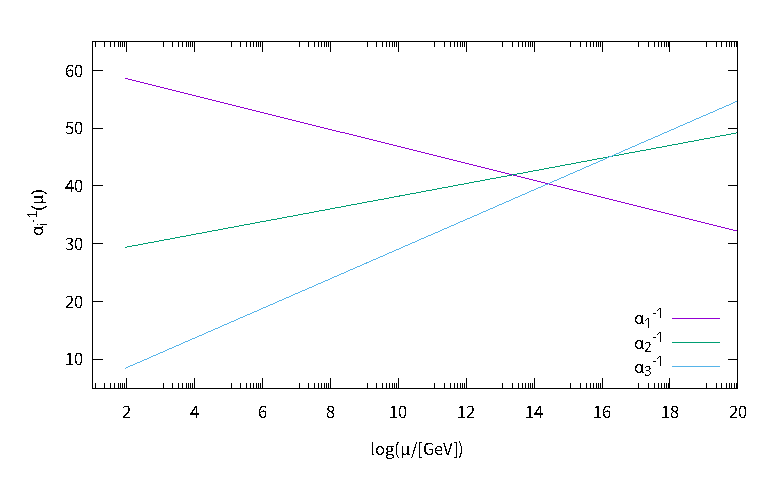
\includegraphics[width=12truecm,clip]{fig/RGE_SM.eps}
  \caption{標準模型粒子のみで繰り込み群方程式を解いた図}
  \label{fig:RGE_SM}
\end{figure}
$\alpha_i$は$\alpha_i(\mu) = \cfrac{g_i(\mu)}{4\pi}$として, 式(\ref{def_beta})に代入し, 
\begin{align}
  \frac{d \alpha_i^{-1}(\mu)}{d\,\mathrm{ln}{\mu}} = -\frac{1}{2\pi}b_i \label{bfnc_1loop}
\end{align}
とする.
電弱スケール $M_Z=91.1880\,[\mathrm{GeV}]$におけるゲージ結合定数の値は
\begin{align}
  g_1(M_Z) &= 0.461\nonumber\\
  g_2(M_Z) &= 0.652\nonumber\\
  g_3(M_Z) &= 1.22\nonumber
\end{align}
であり
\cite{navasReviewParticlePhysics2024}, これらを初期条件として数値的に解いたものが図\ref{fig:RGE_SM}となる.
図\ref{fig:RGE_SM}を見ると明らかであるが, 高エネルギースケールでゲージ結合定数の大きさは近づくものの, 完全には一致しない.
しかし, いずれの相互作用の大きさもプランクスケールである$M_{pl}\sim 10^{19}\,[\mathrm{GeV}]$よりも下で近づくため, 3つの相互作用は重力相互作用よりも先に統一される可能性は残されている.

%EOF


% ----------------------------------------
% 
%  Grand Unified Theory
%  grand_unified_theory.tex
%  Program modified by Yasutoki Takamura
%  Last Modified Jan 10 2025
%
% ----------------------------------------
%\section{大統一理論}
大統一理論はH.GeorgiとS.L.Glashowにより1974年に提唱された\cite{PhysRevLett.32.438}.
大統一理論では重力を除いた3つの相互作用を1つに統一することを目的としている.
したがって, ゲージ対称性は単純群によって記述されると考えられており, 標準模型のゲージ群である$\mathcal{G}_\text{SM}= SU(3)_c\times SU(2)_L\times U(1)_Y$を部分群として内包する群を考える.
このことから, 前節で述べられているような標準模型の問題点はいくつか解決されると考えられている.

\textcolor{red}{要修正: どの点で何が解決できているのか}

大統一理論にも様々な単純群を考えることが可能であり, $SU(5)$や$SO(10)$, $E_6$などの模型を考えることが可能であるが, このノートでは最小模型である$SU(5)$について取り扱い, 理論の拡張を試みる.

はじめに, $SU(5)$大統一理論が最小模型である理由を考える.
標準模型のゲージ対称性である$SU(3)_c\times SU(2)_L\times U(1)_Y$は, 群の階数が$\text{rank}=4$であり, これを内包できる群を考える必要がある.
その中で考えられる単純群は, $\text{O}(8)$, $\mathrm{O}(9)$, $\mathrm{Sp}(8)$, $\mathrm{F}_4$, そして $\mathrm{SU}(5)$である.
このうち, $SU(3)$のもつ3重項をもち, $SU(2)$がもつ2重項の複素表現をもつという性質は$SU(5)$群を用いて記述することができるため, 最小模型として$SU(5)$群を考えて理論を構築することが可能となる.

\section{Georgi-Glashow モデル}
ここから$SU(5)$群を考える.
ゲージ群を決定すると, ラグランジアンに導入する場の既約表現を指定すれば理論を定めることができる.
$SU(5)$の基本表現は$5$表現であり, $5$表現か, その複素表現である$\overline{5}$を用いることですべての表現を構成することができる.
$SU(5)$群の階数は4であるから, 生成演算子を$L_i$$(i=1,\cdots,24)$ のうち対角化可能なものが4つ存在する.
$SU(3)_c$の対角化可能な生成演算子を$\lambda_3,\lambda_8$, $\mathrm{SU}(2)$のものを$I_3$ (アイソスピン), $U(1)$の超電荷を$Y$に対応させて考えることができる.

次にフェルミオンの次元を$\mathrm{SU}(3), \mathrm{SU}(2)$の表現次元, $U(1)$の超電荷$Y$で $(1, 2, -1)$のように表し, どのように$SU(5)$模型に当てはめられるか考える.
\begin{center}
\begin{tabular}{clc}
             &                         & 多重度 \\
  $(u, d)_L$ & $(3  , 2, \frac{1}{6})$ &      6 \\
    $d_L^c $ & $(3^*, 1, \frac{1}{3})$ &      3 \\ 
    $u_L^c $ & $(3^*, 1,-\frac{2}{3})$ &      3 \\ 
$(\nu, e)_L$ & $(1  , 2,-\frac{1}{2})$ &      2 \\ 
     $e_L^c$ & $(1  , 1,           1)$ &      1 \\ 
   $\nu_L^c$ & $(1  , 1,           0)$ &      1 \\ 
\end{tabular}
\end{center}

基本表現をこの中から選ぶことで
\begin{align}
  (q_L^c, \nu_L, e_L) = (3^*, 1, Y)\oplus\left(1,2,-\frac{1}{2}\right) = \overline{5}
\end{align}
と考えられる.
ここではまだ$q$の正体が$u, d$クォークのどちらかは定かではないが, $\mathrm{SU}(5)$群のトレースは0でなければならないため, $Q$を電荷とすると上記の電荷は
\begin{align}
  \sum_{a=1}^5 Q_a = 3Q_{qc}+Q_\nu + Q_e\nonumber\\
  \therefore\quad Q_q = -Q_{qc} = -\frac{1}{3}
\end{align}
となる.
したがって, $q=d$と選択することにより, 次のように$\bm{5}$表現を決めることができる.
\begin{align}
 \bar{\bm{5}}=\begin{pmatrix}
    d_1 ^c \\
    d_2 ^c \\
    d_3 ^c \\
    l      \\
    -\nu_l
  \end{pmatrix}=\left({3}^*,1,\frac{1}{3}\right)\oplus \left(1,2,-\frac{1}{2}\right)\label{GUT-5rep}
\end{align}
これによりクォークの電荷が荷電レプトンの$\frac{1}{3}$の整数倍となっていることが説明できる.
残りのフェルミオンを次元の大きい表現に当てはめることを考える.
基本表現よりも大きな表現は, すべて基本表現の積で表すことができる.
${\bm{10}}$表現は
\begin{align}
  \bm{5}\otimes\bm{5} = \bm{15}\oplus\bm{10}\nonumber
\end{align}
として構成することができる.
この$\bf{10}$表現は$\bm{10}\rightarrow (3^*,1,-\frac{2}{3})\oplus(3,2,\frac{1}{6})\oplus(1,1,1)$
と分解できるので, 次のように当てはめることができる.
\begin{align}
  \overline{\bm{10}}= \frac{1}{\sqrt{2}}\begin{pmatrix}
         0 &  u_3^c & -u_2^c & u_1 & d_1 \\
    -u_3^c &      0 &  u_1^c & u_2 & d_2 \\
     u_2^c & -u_1^c &      0 & u_3 & d_3 \\
    -u_1   &   -u_2 &   -u_3 &   0 & e^c \\
      -d_1 &   -d_2 &   -d_3 &-e^c &   0 \\
    \end{pmatrix}\label{GUT-10rep}
% Note
% 10表現であれば内部に規格化定数を入れる場合があるがここで必要ではないのか確認しなければならない.
% Dec 10: up quark massを出す際に規格化されている必要があるので, この規格化定数は必要.
\end{align}
ただし, $x^c$は$x$を同じカイラリティで荷電共役したものを表している.
この$x$の例として, 左巻きの電子$e^-_L$を考える.
$e^-_L$に対して荷電共役変換を行った$(e^-_L)^c$を考える.
これは右巻きの電子$e_R^-$となるが, 左巻きの陽電子である$e_L^+$と同じである.
\subsection{ゲージ粒子の表現}
$SU(n)$ゲージ理論では, $n^2-1$個のゲージ場が存在する.
$SU(5)$群の生成演算子を, $[L_i]^a_b\,(i=1,\cdots,24, a,b=1,\cdots,5)$として構成する.
基本表現である$5$表現の類推からは$a,b=1,2,3$はカラー量子数, $a,b=4,5$がアイソスピン量子数と考えられる.
そのため$i=1,\cdots,8$を$SU(3)$部分, $i=9,10,11$を$SU(2)$の部分群として考えると
\begin{align}
  L_i(i=1,\cdots,8) = \left(\begin{array}{ccccc}
        &           &   & 0 & 0 \\
        & \lambda_i &   & 0 & 0 \\
        &           &   & 0 & 0 \\
      0 &         0 & 0 & 0 & 0 \\
      0 &         0 & 0 & 0 & 0 
  \end{array}\right),\quad
  L_i(i=9,10,11) = \left(\begin{array}{ccclcc}
      0 &  0 & 0 & & 0 & 0 \\
      0 &  0 & 0 & & 0 & 0 \\
      0 &  0 & 0 & & 0 & 0 \\
      0 &  0 & 0 & & \sigma_i      \\
      0 &  0 & 0 & &       \\
  \end{array}\right),\quad
\end{align}
24個のゲージボゾンは随伴表現として存在し, 次のように分解できる.
\begin{align}
  \bm{24} = G^i(8,1,0)\oplus W^i(1,3,0)\oplus B(1,1,0)\oplus \bar{X}(3,\bar{2},-\frac{5}{6})\oplus X(\bar{3},2,+\frac{5}{6})
\end{align}
ゲージボゾンを$V_\mu$とすると,
\begin{align}
  \frac{1}{\sqrt{2}}V_\mu &= \sum_{i=1}^{24}\frac{1}{2}V_\mu^i L_i\\
  V_\mu &= \left(\begin{array}{ccccc}
    G^1_1 - \frac{2B}{\sqrt{30}} & G^1_2 & G^1_3 & \bar{X_1} & \bar{Y_1} \\
    G^2_1 & G^2_2 - \frac{2B}{\sqrt{30}} & G^2_3 & \bar{X_2} & \bar{Y_2} \\
    G^3_1 & G^3_2 & G^3_3 - \frac{2B}{\sqrt{30}} & \bar{X_3} & \bar{Y_3} \\
    X_1   & X_2 & X_3 & \frac{W^3}{\sqrt{2}} + \frac{3B}{\sqrt{30}} & W^+ \\
    Y_1   & Y_2 & Y_3 & W^- &    -\frac{W^3}{\sqrt{2}} + \frac{3B}{\sqrt{30}} 
      \end{array}
  \right)
\end{align}
ただし, $SU(3)$ゲージ場の部分は$G^i\,(i=1,\cdots,8)$をグルーオン場として
\begin{align}
  G^1_2 = G^1,\quad G^2_1 = G^2,\quad G^3_1 = G^5,\quad G^2_3 = G^6,\quad G^3_2 = G_7\nonumber\\
  G^1_1 = \frac{G^3}{\sqrt{2}} + \frac{G^8}{\sqrt{6}},\quad G^2_2=-\frac{G^3}{\sqrt{2}}+\frac{G^8}{\sqrt{6}},\quad G^3_3 = -\frac{2G^8}{\sqrt{6}}\nonumber
\end{align}
であり, $SU(2)$ゲージ場は
\begin{align}
  W^\pm = \frac{W^1\mp iW^2}{\sqrt{2}}\nonumber
\end{align}
である.
\subsection{対称性の破れ}
\subsection{予言される現象}
\subsection{破綻}


%EOF


% ----- 2nd part -----
%\part{研究の部分}

\chapter{SU(5)大統一理論の拡張模型}
% ---------------------------------------
%
%  Extend to SU(5) GUT
%  extend_SU5.tex
%  Program modified by Yasutoki Takamura
%  Last Modified Jan 21 2025
%
% ---------------------------------------
\section{高次元表現ヒッグスを用いた拡張}
15表現ヒッグスを

%EOF


\newpage
\noindent
{\large \bf{結論}}

% ---------------------------------------
%
%  Conclusion
%  conclusion.tex
%  Program modified by Yasutoki Takamura
%  Last Modified Jan 27 2025
%
% ---------------------------------------
本論文では素粒子標準模型がどのような理論体型であったのか確認し, さらに標準模型では説明できない物理現象を簡単にまとめた.
その中でも場の理論による繰り込みという手法を用いることで,  ゲージ結合定数の大きさはエネルギー依存性をもち, 3つのゲージ結合定数の大きさは高いエネルギーになるにつれて近づくことがわかった.

標準模型ではゲージ対称性によって相互作用が記述される.
大統一理論はそのゲージ対称性を高いものへ拡張し, 標準模型を部分的に含むことによって理論を構築するものであり, 非常に自然な拡張だと考えられる.

最小$SU(5)$大統一理論は陽子崩壊が観測されていないため実験的に排除されてしまっているが, 単純群で標準模型を含むアイデアは画期的なものであり, 拡張の余地がある.

本論文では$\bm{15}$表現ヒッグスを加えることでくりこみ群方程式の係数が実際に変化し, ゲージ結合定数が統一される様子を確認できた.
このように電弱スケールと大統一スケールの間に粒子が存在する場合, 最小$SU(5)$模型では叶わなかったゲージ結合定数の大きさを統一する可能性が高まる.
しかし, そのような中間スケールに粒子の存在する場合, 新粒子の性質によっては陽子の崩壊を非常に早めてしまう可能性もある.
本論文ではそのような解析まで行えていないが, 低スケールに$\bm{15}$表現ヒッグスのレプトクォーク成分が存在しているため, 既にこの模型も実験的に棄却され始めている\cite{collaborationSearchProtonDecay2020}.

一方で, ニュートリノが質量を持つことは実験的に揺るぎないものであり, タイプII型のシーソー機構を含むような拡張を標準模型に施すのであればスカラー三重項を理論に加える必要がある.
そのような拡張を有効演算子として加える場合であっても, 高いゲージ対称性を持つ大統一理論がそのような粒子を含む必要があるため, $SU(5)$大統一理論に対して$\bm{15}$表現ヒッグスを加えた拡張を行い研究を行うことは意義があると考える.

今後の研究では$\bm{15}$表現ヒッグスが$SU(5)$大統一理論に拡張され, 陽子崩壊の制限を回避し, ニュートリノ質量が観測事実と整合性のとれた説明ができる模型の探査を行う.
本論文で述べたように$SU(5)$大統一模型が持つ問題点はニュートリノ質量以外にもいくつか存在していた.
それらを解決できるような模型を考案することを今後の研究としたい.



% ----- Appendix -----
\appendix
\chapter{群論}
% ---------------------------------------
%
%  Group theory
%  group_theory.tex
%  Program modified by Yasutoki Takamura
%  Last Modified Jan 27 2025
%
% ----------------------------------------
この章では, 大統一理論に必要な数学の内容を非常に簡単にまとめた.
本文でもほとんど触れられているが, 数学の部分のみを取り出してまとめている.
次のことを認め, 話を進める.

$X$を集合とする.
写像$\phi: X\times X \rightarrow X$のことを集合$X$上の演算と言う.
これ以降では$a,b,\in X$に対する写像を$\phi(a, b)$の代わりに$ab$と書く.
\section{群}
群とは次の性質を持つものである.
\begin{dfn}[群]
  $G$を空ではない集合とする. 集合$G$上で演算が定義されており, 次の性質を満たすとき, $G$を群と言う.
  \begin{enumerate}
    \item 単位元と呼ばれる$e\in G$が存在し, 全ての$a\in G$に対して$ae=ea=a$となる.
    \item すべての$a\in G$に対し, $b\in G$が存在し, $ab=ba=e$となる. この元$b$は$a$の逆元と呼ばれ, $a^{-1}$と書く.
    \item すべての$a, b, c \in G$に対して, $(ab)c=a(bc)$が成り立つ.
  \end{enumerate}
\end{dfn}
特に, 性質3. は結合法則と呼ばれている.
群の元$a, b\in G$に対して$ab=ba$が成り立つとき, $a, b$は可換である.
$G$の任意の元$a, b$が可換なら, $G$を可換群(Abel群)と呼ぶ.
\section{Lie群}
Lie群は連続なパラメータにより特徴づけられる群であり, 生成子$t^a$によって
\begin{align}
  g(\alpha) = \exp(i\alpha^a t^a)
\end{align}
となる.
この生成子$t^a$は, リー括弧によって
\begin{align}
  [t^a, t^b] = if^{abc}t^c
\end{align}
を満たす.
ここで, $f^{abc}$はリー代数の構造定数である.
\section{表現}
表現とは, 群を行列に対応させる写像である.
この写像は$\mathcal{R}: G\rightarrow GL(n)$で定義される.
表現の次元は行列の次元と等しい.


%EOF



\chapter{標準模型でのくりこみ群方程式の係数の計算}
$B$3$3$G$O%2!<%87k9gDj?t$K4X78$9$k$/$j$3$_72J}Dx<0$r(B, $BI8=`LO7?N3;R$G$I$N$h$&$K(B$b_i$$B$r7W;;$7$?$+5-O?$9$k(B\cite{royCalculating$v$functionCoefficients2019}
$B$3$3$G$ONL;RJd@5$N(B1$B<!$N9`$^$G$N$_$r9M$($F$$$k(B.


Dynkin$B;X?t(B$S(R)$$B$O4{LsI=8=$rMQ$$$F<!$N$h$&$KDj5A$5$l$k(B.
\begin{align}
 \mathrm{Tr}[S^aS^a] = S(R_i)\delta^{ab}
\end{align}
$SU(N)$$B72$K$*$1$k4pK\I=8=$KBP$7$F(B, $B0lHLE*$K(B$S(R) = \frac{1}{2}$$B$H5,3J2=$5$l$k(B.
$B$^$?(B, $B%+%7%_%"1i;;;R(B$C_2(R)$$B$H(BDynkin$B;X?t$K$D$$$F$O(B
\begin{align}
  d(G)S(R) = d(R)C_2(R)
\end{align}
$B$HBP1~IU$1$i$l$k(B.
$B$3$3$G(B, $d(R)$$B$OI=8=(B$R$$B$N;~E@$G$"$j(B, $d(G)$$B$O%2!<%872(B$G$$B$N?oH<I=8=$N<!85$G$"$k(B.

$B$3$3$+$iI8=`LO7?$N>l9g$I$N$h$&$J7W;;$,$5$l$k$+<B:]$K8+$k(B.
\begin{align}
  C_R^3 (i) = \left\{\begin{array}{cc}
      \cfrac{4}{3} & \Psi = Q, \bar{u},\bar{d} \\\\
      0 & \Psi_i L, \bar{e}, H
  \end{array} \right.\nonumber\\
  C_R^2 (i) = \left\{\begin{array}{cc}
      \cfrac{3}{4} & \Psi = Q, L, H \\\\
      0 & \Psi_i = \bar{u}, \bar{d}, \bar{e}
  \end{array} \right.\nonumber\\ 
  C_R^3 (i) = \begin{array}{cc}
    \cfrac{3Y^2_i}{5}& \text{$BD6EE2Y$NCM$r2C$($k(B.}
  \end{array}\nonumber
\end{align}

$B$^$?(B, Dynkin$B;X?t$K$D$$$F$b(B
\begin{align}
  S_2(R) = \left\{ \begin{array}{cc}
      \cfrac{3}{5}Y^2_{\Psi_i} & U(1) \\\\
      \cfrac{1}{2} & SU(N)
    \end{array}\right.
\end{align}
$B$H$J$k(B.
$B$3$l$rF'$^$($F<B:]$K?t$r4*Dj$9$k$H<!$N$h$&$K$J$k(B.
\begin{eqnarray}
\label{b1funcSM}
b_1 &=&0+\frac{4}{3}\cdot\frac{1}{\tikzmark{b1SM1}2}\cdot\bigg(\sum_{\mathrm{fermions}}\frac{3}{5}Y_{\mathrm{fermions}}^2\bigg)+\frac{1}{6}\cdot\tikzmark{b1SM2}2\cdot\bigg(\sum_{\mathrm{scalars}}\frac{3}{5}Y_{\mathrm{scalars}}^2\bigg)~~[\mathrm{$B$?$@$7(B}~ U(1), C_2(G)=0]\nonumber\\\nonumber\\
&=& \frac{2}{3}\cdot\sum_{\mathrm{fermions}}\frac{3}{5}Y_{\mathrm{fermions}}^2+\frac{1}{3}\cdot\sum_{\mathrm{scalars}}\frac{3}{5}Y_{\mathrm{scalars}}^2 \nonumber\\\nonumber\\
&=& \frac{2}{5}\bigg[\tikzmark{b1SM3}(3\cdot\tikzmark{b1SM4}2)\cdot(\frac{1}{6})^2+(3\cdot 1)\cdot(-\frac{2}{3})^2+(3\cdot 1)\cdot(\frac{1}{3})^2+\tikzmark{b1SM5}2\cdot(-\frac{1}{2})^2+\tikzmark{b1SM6}1\cdot 1^2\bigg]N_f+ \frac{1}{5}\bigg[2\cdot(-\frac{1}{2})^2\bigg]N_H \nonumber\\
\begin{tikzpicture}[remember picture,overlay]
\draw[<-] 
  ([shift={(2pt,-2pt)}]pic cs:b1SM1) |- ([shift={(-14pt,-12pt)}]pic cs:b1SM1) 
  node[anchor=east] {$\scriptstyle \text{Weyl fermion}$}; 
\draw[<-] 
  ([shift={(2pt,-2pt)}]pic cs:b1SM2) |- ([shift={(-14pt,-14pt)}]pic cs:b1SM2) 
  node[anchor=east] {$\scriptstyle \text{Complex scalar}$};   
\draw[<-] 
  ([shift={(2pt,-2pt)}]pic cs:b1SM3) |- ([shift={(-14pt,-14pt)}]pic cs:b1SM3) 
  node[anchor=east] {$\scriptstyle \text{Color}$}; 
\draw[<-] 
  ([shift={(2pt,-2pt)}]pic cs:b1SM4) |- ([shift={(16pt,-16pt)}]pic cs:b1SM4) 
  node[anchor=west] {$\scriptstyle \text{Doublet}$}; 
\draw[<-] 
  ([shift={(2pt,-2pt)}]pic cs:b1SM5) |- ([shift={(16pt,-16pt)}]pic cs:b1SM5) 
  node[anchor=west] {$\scriptstyle \text{Doublet}$}; 
\draw[<-] 
  ([shift={(2pt,-2pt)}]pic cs:b1SM6) |- ([shift={(16pt,-16pt)}]pic cs:b1SM6) 
  node[anchor=west] {$\scriptstyle \text{Singlet}$}; 
\end{tikzpicture}
&=& \frac{4}{3}N_f+\frac{1}{10}N_H 
\end{eqnarray}
$B$?$@$7(B, $N_f$$B$O%U%'%k%_%*%s$N@$Be?t$G$"$j(B, $N_H$$B$O%R%C%0%9Fs=E9`$N?t$G$"$k(B.
$BF1$8$h$&$K(B$b_2$$B$b7W;;$9$k$H<!$N$h$&$K$J$k(B.
\begin{eqnarray}
\label{b2funcSM}
b_2 &=& \frac{2}{3}\cdot\frac{1}{2}\big[(\tikzmark{b2SM1}3\cdot 1)+(1\cdot 1)\big]N_f+\frac{1}{3}\cdot\frac{1}{2}(1\cdot 1)N_H-\frac{11}{3}\cdot 2
\begin{tikzpicture}[remember picture,overlay]
\draw[<-] 
  ([shift={(2pt,-2pt)}]pic cs:b2SM1) |- ([shift={(14pt,-14pt)}]pic cs:b2SM1) 
  node[anchor=west] {$\scriptstyle \text{Color}$}; 
\end{tikzpicture}
\nonumber\\
&=& \frac{4}{3}N_f+\frac{1}{6}N_H-\frac{22}{3}.
\end{eqnarray}

$B:G8e$K(B$b_3$$B$K$D$$$F$b<!$N$h$&$K7W;;$5$l$k(B.
\begin{eqnarray}
\label{b3funcSM}
b_3 &=& \frac{2}{3}.\frac{1}{2}(\tikzmark{b3SM1}2+1+1)N_f-\frac{11}{3}.3
\begin{tikzpicture}[remember picture,overlay]
\draw[<-] 
  ([shift={(2pt,-2pt)}]pic cs:b3SM1) |- ([shift={(14pt,-14pt)}]pic cs:b3SM1) 
  node[anchor=west] {$\scriptstyle \text{Doublet}$}; 
\end{tikzpicture}
\nonumber\\
&=& \frac{4}{3}N_f-11,
\end{eqnarray}
%EOF


\newpage
\noindent
{\large \bf{謝辞}}

この世を複雑に作った神に感謝.

% ----- Bibliography -----
\bibliographystyle{junsrt}
\bibliography{
bibs/GUT.bib,
bibs/Standard_Models.bib,
bibs/CS_Equation.bib,
bibs/Glashow_Weinberg.bib,
bibs/QCD.bib,
bibs/beta_function.bib,
bibs/Experimental.bib,
bibs/neutrino_oscillation.bib,
bibs/neutrino_oscillation_th.bib,
bibs/Leptoquark.bib,%
bibs/SU5_45Higgs.bib,%
bibs/CKM.bib, % Cabbibo Kobayashi Masukawa Matrix
bibs/CP_violation.bib, % Chronin fitch 
bibs/BEGN.bib,
bibs/GUT_others.bib,
bibs/mdmsmass.bib,
bibs/15rep.bib,
bibs/proton_stability.bib,
bibs/no_p.bib,
bibs/b_calc.bib
}

\end{document}
%EOF
